\section{Visualization} % (fold)
\label{sub:visualization}

The greatest challenge of this work was the creation of the visualization part for its requirements. We will now describe this part of Eagle Eye, its architecture, visualization techniques, sorting and filtering capabilities.

\subsection{Overview}
We wanted to make the visualization simple and easy to use, while keeping it flexible and capable enough to allow for an enjoyable and relevant experience.

After the backend has finished the all the processing that is needed, the visualization can be opened and all images that were added to the backend's processing list will appear in what we call ``the canvas''. After loading the metadata, the user is also presented with a set of options on the top toolbar, which contains all the controls needed to use the system (\fig{viz5679images}).


\begin{figure}[ht]
	\centering
		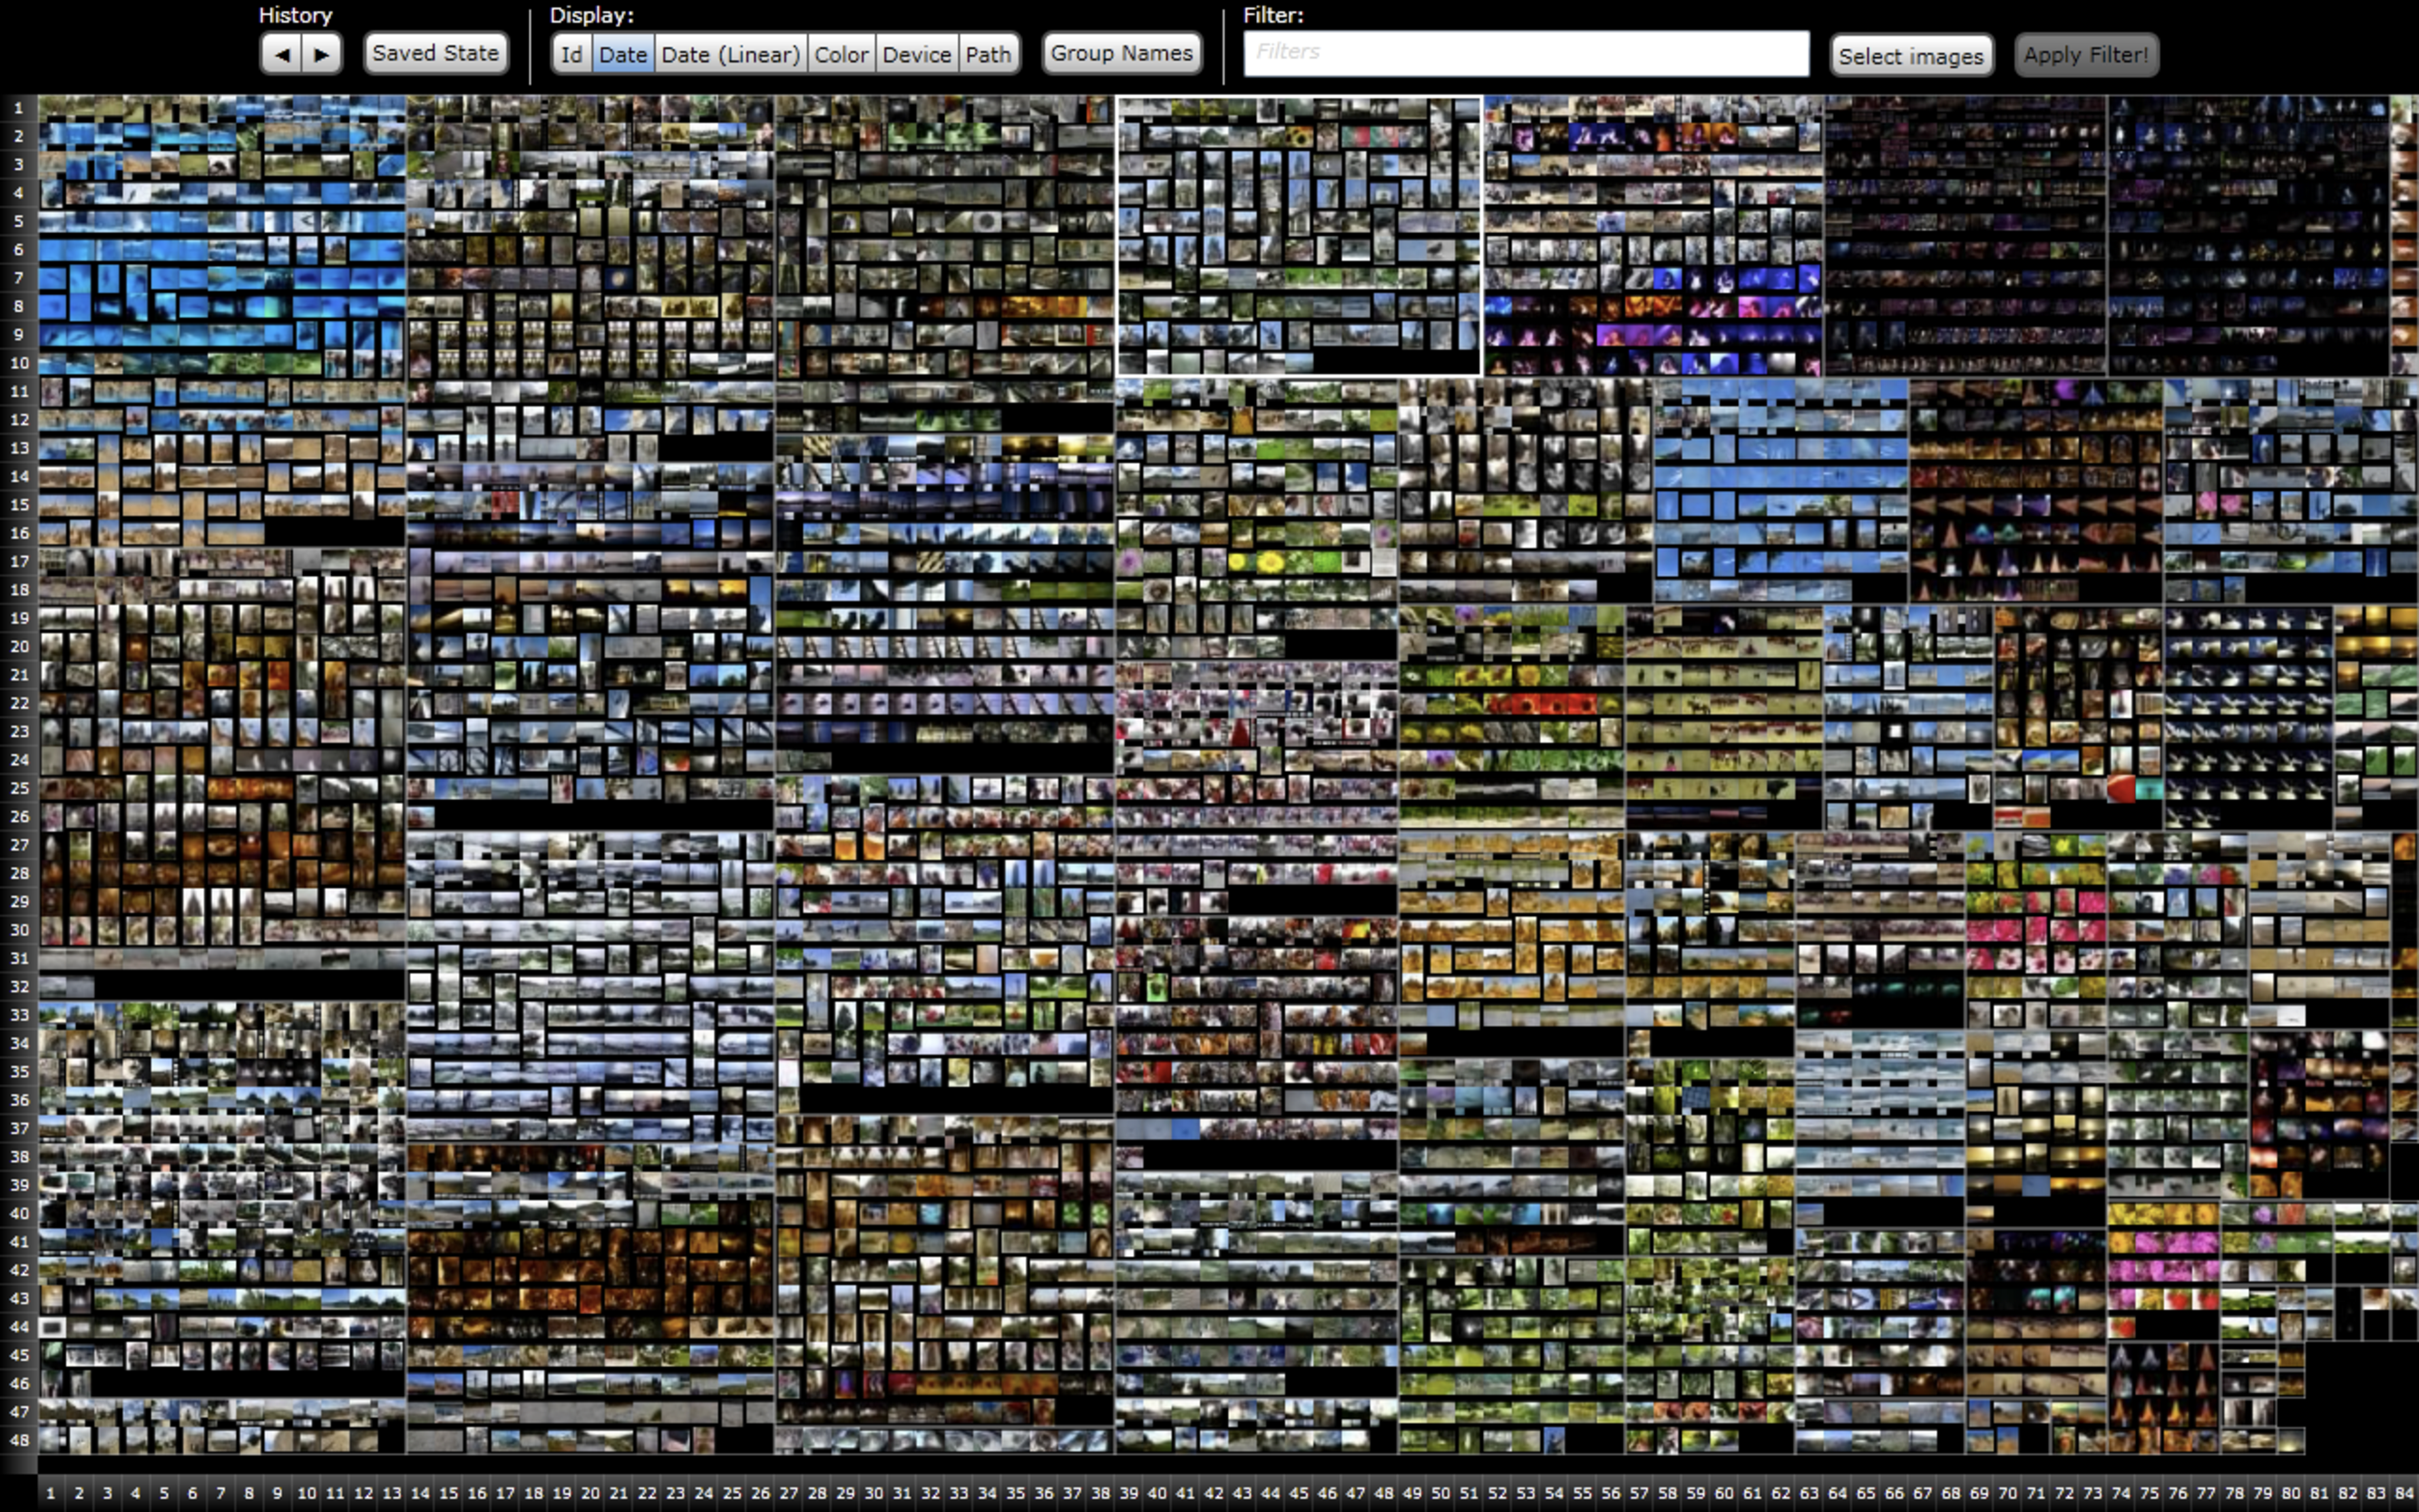
\includegraphics[width=\columnwidth]{Figures/viz5679images1280.pdf}
	\caption{Example of the visualization of 5679 images, organized by capture date, in Eagle Eye.}
	\label{fig:viz5679images}
\end{figure}



\subsubsection{The Canvas}

The canvas is the most relevant part of the visualization as it displays the user's images.

According to A. Torralba \cite{Torralba:2008p527}, an image with 32 pixels per side is the minimum size that allows a user to recognize what it is. His work was about an image library that had nothing to do with the user's photo. On Eagle Eye, we can have even smaller images because our focus is the user's own library. This allows much easier recognition of images since, by looking at the form and colors, the user recalls what is that image without having to ``read'' and understand a totally new image. Another very important help is the grouping of events (e.g. by date or path) which allows the user to extrapolate the contents of the whole group from looking at a few of them instead of trying to understand each image individually. This allows much faster recognition of groups with images at really small sizes, even if not all images can be understood.

An example of this can be seen on figure \ref{fig:viz5679images}, which is a screenshot of the application running on a 13.3" screen with a resolution of 1280x800 pixels, where the larger side of each image uses 15 pixels and takes 3 millimeters. On this example, different groups are clearly distinguishable from each other and most of them are easily recognizable by the owner of the photographs. Each group seems to have a specific set of colors, e.g., blue, green, yellow, orange, gray or black, making easy for the owner to distinguish and recognize the photos.

A photo application that only displays all images isn't very useful, therefore, manipulation of the canvas is allowed by zooming and panning. This means the user can, at any time, use the mouse to drag the canvas around or, by clicking or scrolling, zoom in and out of the canvas. Zooming goes from the default view of thousands of images at the same time, to the full screen view of one of them, and everything in between in a smooth way. This allows a closer look to any group or image, providing an easy and fluid way to navigate the collection.


%%%%%%%%%%%%%%%%%%%%%%%%%%%%%%%%
\subsubsection{The toolbar}

\begin{figure}[htbp]
	\centering
		
\includegraphics[width=\linewidth]{Figures/toolbar.png}
	\caption{The toolbar on top of the visualization \ac{UI}.}
	\label{fig:toolbar}
\end{figure}


The user can then use the functions on the toolbar to filter and sort differently. The toolbar is divided in three sections: History, Display and Filtering (\fig{toolbar}).

The History section contains some basic functions that work similarly to the current web browsers. There are buttons for going back and forward between the history of display states and a save button for bookmarking the current display state, allowing the user to easily get back to it later.

The Display section, in the middle contains two options to change the image display: the sorting options and the display overlays button. The former presents the available sorting options for the current collection, based on the available metadata and on the best ways to display them. The content is presented according to the selected option and changing to another causes the images on display to move around to a new position and form a different display order. This sorting and disposition options will be explained in a later section.
The other button in this section of the toolbar is called ``Group Names'' and enables or disables a layer of information on top of the images. This layer distinguishes the groups of images in display by painting them with different colors and presenting names for them, depending on the selected sort option (\fig{overlays} shows an example of this). Grouping will also be explained bellow. 

\begin{figure}[htbp]
	\centering
		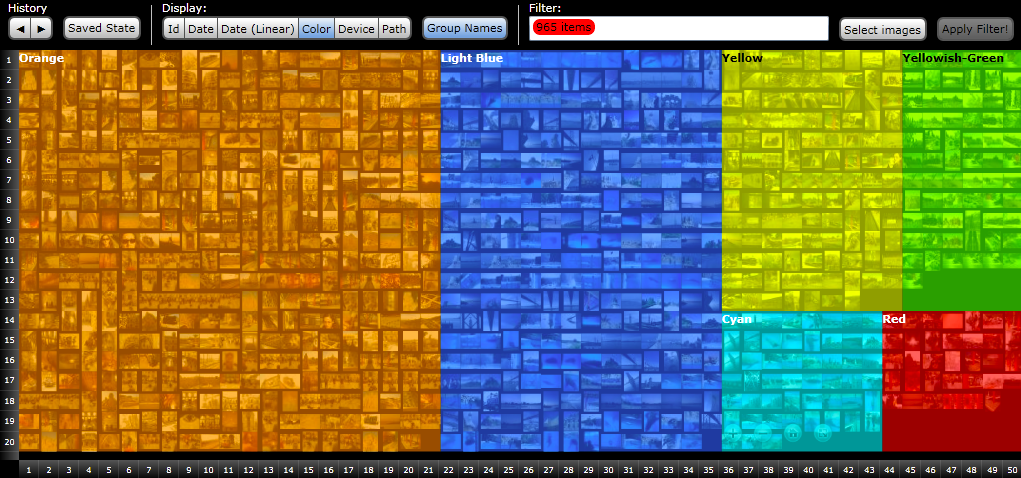
\includegraphics[width=\linewidth]{Figures/overlays.png}
	\caption{By enabling overlays, the user can see names for the groups and a much more clear group distintion.}
	\label{fig:overlays}
\end{figure}

The third and final section of the toolbar is the filter section. It contains controls to filter images by using simple text and to visually select images on the canvas. This options will also be explained bellow.



\subsection{Disposition of Images on Canvas}
\label{sub:dispositions}

The different ways to dispose the images on the canvas was a matter that required some exploration of possibilities, like the ones seen on the Related Work (\cite{Bederson:2001:PZI:502348.502359,Bruls:2000p3517,Chen:1998p2344,Girgensohn:2010,Heesch:2004p2675,Hsu:2009p2696,Porta:2006p416,Rodden:2001p731,Schaefer:2010p1871,Strong:2009p413}).

We have come up with a some options for photo grouping, sorting and filtering. We kept a sensible set of the choices so its easy and understandable for users. 
To make sense of how all this pieces work together, we are going to explain how do we sort images into groups and the different ways the user can arrange those groups on the canvas, followed by how filtering is done.


\subsubsection{Sorting images into groups}

As we've seen previously, the backend outputs metadata for each image. This set of metadata is loaded into the visualization application of Eagle Eye and is then indexed by type.

For instance, each image has an associated creation timestamp which will be aggregated by days, generating an image group for each day.

Similarly, the mean color associated with each image is indexed and groups are generated by splitting the hue spectrum. We used a quick approach and divided it into 12 equal bins with names, as can be seen in figure \ref{fig:colorbins}. From the image, it's possible to see that some colors have a greater usage of the spectrum, like green, which takes the most part of three bins, while other colors use only one. This gives the user multiple tones for some colors and only one for others. We made it this way so the number of bins could be quickly changed to something else if we saw fit but the most sensible option might have been to manually define the bins with different sizes and more accurate names.

\begin{figure}[htbp]
	\centering
		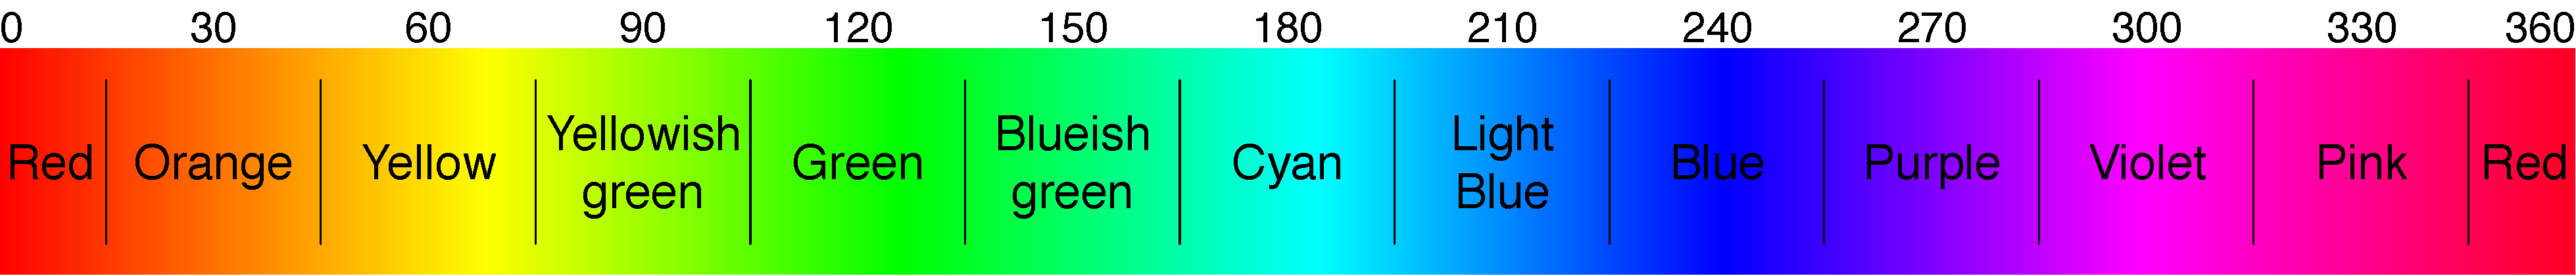
\includegraphics[width=\linewidth]{Figures/colorbins}
	\caption{Division of the hue values in 12 equal parts, 30 points apart from each other.}
	\label{fig:colorbins}
\end{figure}

Another option is the grouping by device name, which usually allows to distinguish between who took the pictures if, for instance, different people have different cameras on the same event.

The last option currently available to the user is grouping by path which groups together the images that were already grouped by the user, on the file system. This allows for the display of an organization that is recognizable to the user, which can make a good starting point.

On the canvas, group boundaries are identifiable by discrete gray borders and, when the Show Overlays function is active, by color rectangles that also contain the groups' names.


\subsubsection{Different dispositions}

After having the images grouped by any of the sorting options referred on the previous section, the system has to know how to display them on the canvas.

We looked into various options (\cite{Bederson:2001:PZI:502348.502359,Bruls:2000p3517,Chen:1998p2344,Girgensohn:2010,Heesch:2004p2675,Hsu:2009p2696,Porta:2006p416,Rodden:2001p731,Schaefer:2010p1871,Strong:2009p413}) and picked the concepts that we thought that made sense and that would be easier for the user to understand. We chose a treemap view and a column-based linear view. Both of these are grid-based layouts, meaning that images are positioned inside a defined grid on the canvas. We also looked into free positioning systems (\cite{Girgensohn:2010,Rodden:2001p731,Schaefer:2010p1871,Strong:2009p413}) but they make it harder for the user to understand the images within, since some images will be covered by others. When displaying thousands of images, it's important to make them easy to see, and mixing them up wasn't the appropriate thing to do. We focused on other ways for making it easier to the user see what matters and we will talk about them later on.

\begin{wrapfigure}{r}{0.4\textwidth}
	\vspace{-23pt}
	\begin{center}
		\includegraphics[width=0.39\textwidth]{Figures/Protovis-treemap.pdf}
	\end{center}
	\vspace{-20pt}
	\caption{Common treemap based on space filling.}
	\vspace{-5pt}
	\label{fig:commontreemap}
\end{wrapfigure}

The first layout technique we employed was the treemap. Introduced by Brian Johnson and Ben Shneiderman \cite{Johnson:1991:TSA:949607.949654} in 1991, treemaps recursively subdivide areas into rectangles. The problem is that areas can take many forms, from squares or large rectangles to almost thin lines, like can be seen on \fig{commontreemap}. Applying treemaps to images calls for the adaptation of the algorithms to make sure the areas can correctly hold the images and that all images in all groups have the same size and are positioned in the same grid, to make them easier to view. This ideas are supported by B. Bederson on his work with the Quantum Treemaps \cite{Bederson:2001:PZI:502348.502359}. We tried to apply quantum treemap as our treemap algorithm but, due to its complexity and other recurring problems, we had to move to a simpler method and adapted the squarified treemaps \cite{Bruls:2000p3517} by Mark Bruls to support the grid of images that we required. This algorithm was much easier to understand, adapt and implement.

Our resulting treemap algorithm displays larger groups first, leaving the smaller ones to the end, making an effort to layout groups as rectangles with an aspect ratio as close as possible to the screen's aspect ratio, for filling the screen when the user zooms on one. There's also an effort to fill the space left between larger groups and the edges of the screen, making the display more compact and with less empty space across the screen edges.

\begin{figure}[!htb]
  \begin{subfigmatrix}{2}
    \subfigure[Images only.] {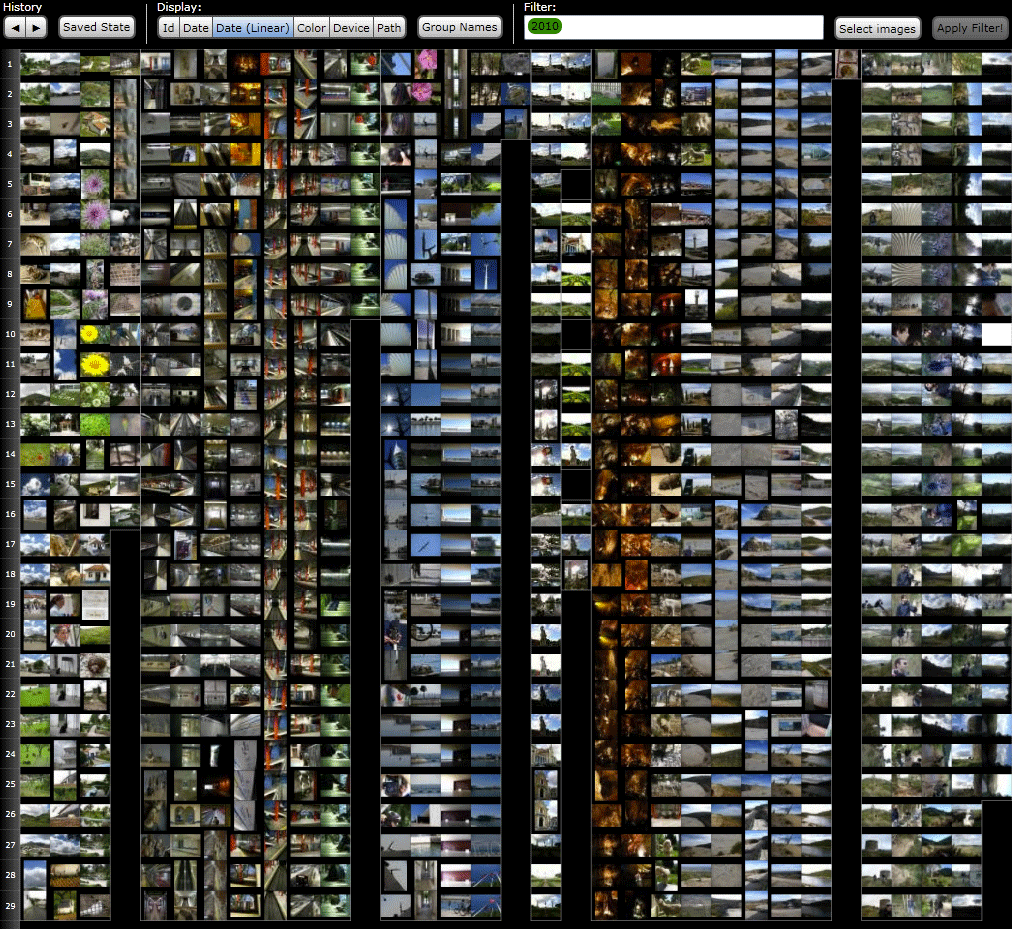
\includegraphics[width=0.49\linewidth]{Figures/linear-2010-thin-1.png}\label{fig:linear1}}
    \subfigure[With group divisions overlayed.]{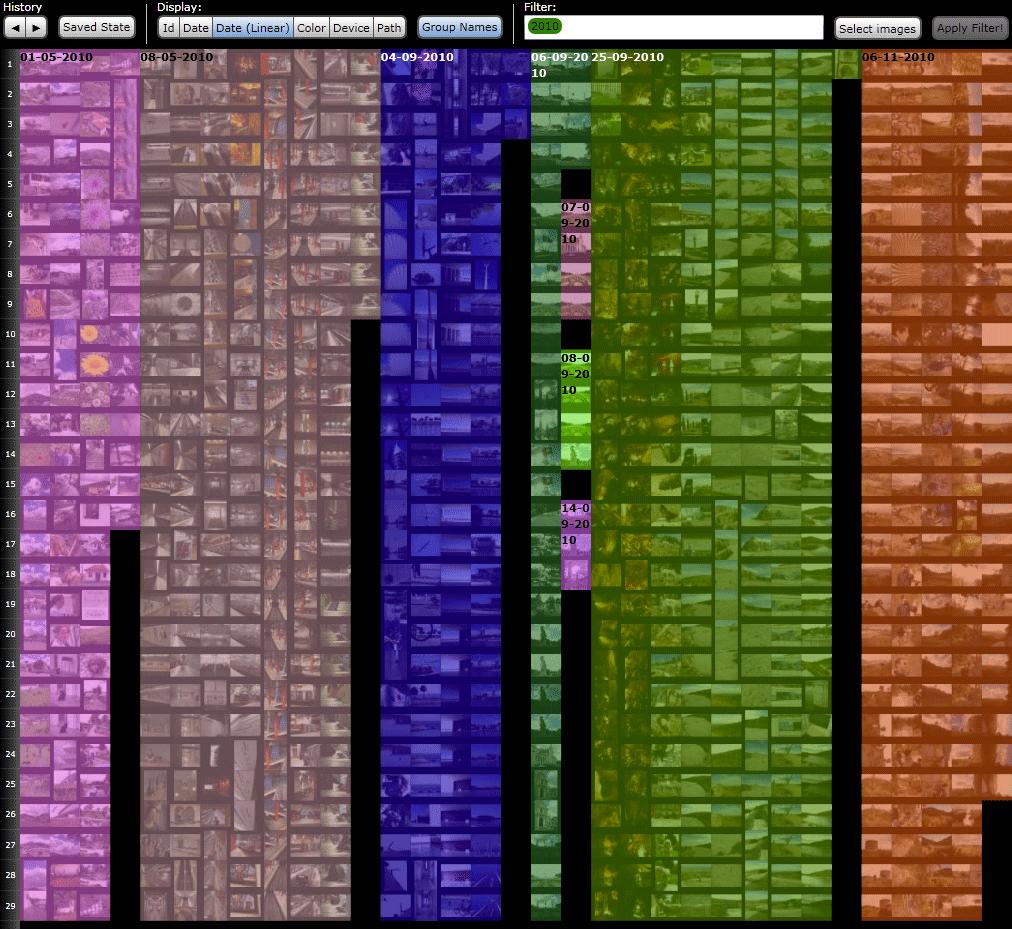
\includegraphics[width=0.49\linewidth]{Figures/linear-2010-thin-2.png}\label{fig:linear2}}
  \end{subfigmatrix}
  \caption{Example of the linear display.}
  \label{fig:linear}
\end{figure}

One problem of the squarified treemap display is that group sequence is irrelevant. Groups are positioned by their size, which is unacceptable for sorting options that require some sequence, like sorting by time. For this we created a linear display (\fig{linear}) that uses columns and displays groups sequentially. Each group may fill part of a column or various columns, depending on their size. With the aim of reducing wasted space, groups that fit on the wasted space left by the previous group use that space to display themselves. This is useful to group the few pictures the users may capture of their day-to-day, between days (like weekends) that he went on a trip and took a much larger number of photographs.

Currently we are using this layout system only for the date display since the use of columns makes visualization harder, requiring either some panning from top to bottom or selecting the group using the filter tools explained ahead. This is an area we must improve, and we will discuss some ideas later on.


\subsubsection{Filtering} % (fold)
\label{ss:filtering}

In addition to the sorting options explained above, Eagle Eye also provides the user with the ability to filter images. This allows the users to focus on specific groups of pictures that are of interest at a particular moment.

For instance, the user might want to only see photos of a day, or a person, or person in a specific day or even pictures that are mostly blue.

For all this, Eagle Eye provides two ways to specify this kinds of constraints: using the filter bar or selecting pictures on the canvas, and we will now look into both them.

The filter bar's purpose mimics a regular search box, similar to the ones that exist on applications like internet browsers, file browsers or photo browsers: it provides a way for the user to type what he is looking for and get some suggestions to help him with the search. Since we wanted a simple \ac{UI}, we figured that we had to provide smart suggestions to the user, so that he can feel comfortable using it for multiple types of searches. Searches are performed immediately upon selecting the desired filter. Currently, searches are only intersections (commonly ``and'') of the entries in the filter bar but after adding adequate \ac{UI}, it will be possible to also use unions (commonly ``or'').

Every piece of the metadata can be used as a filter and the suggestions list shows what are the available options and what type of metadata they relate to, for instance, when looking for a person's name, the ``keyword'' metadata type is shown, when searching for a place, both ``keyword'' and ``path'' types might be presented, if the path to the pictures included the place where they were taken.

\begin{wrapfigure}{r}{0.35\textwidth}
	\vspace{-20pt}
	\begin{center}
		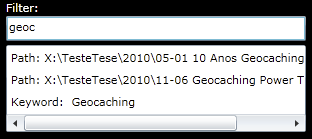
\includegraphics[width=0.34\textwidth]{Figures/filter_0000_geoc.png}

		\vspace{7pt}

		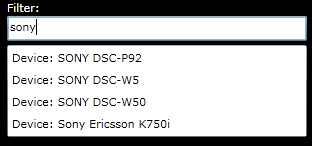
\includegraphics[width=0.34\textwidth]{Figures/filter_0001_sony.png}

		\vspace{7pt}

		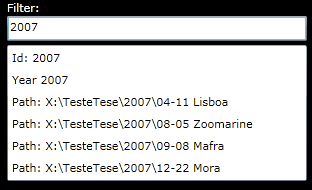
\includegraphics[width=0.34\textwidth]{Figures/filter_0004_2007.png}
	\end{center}
	\vspace{-25pt}
	\caption{Examples of filter suggestions.}
	\vspace{-5pt}
	\label{fig:filter}
\end{wrapfigure}

This examples are quite simple but we wanted to go further and allow searches like ``Summer'', for all photos taken around the summer time in all years, ``May 2010'', for all pictures taken during that month, ``Has 2 people'' for photos that have been detected to have people in them. Although some of these examples have not been fully implemented yet, they are in the plans. See figure \ref{fig:filter} for some examples.

The second filter method allows the manual selection of images from the canvas, either by a common mouse drag-and-drop on the canvas or by selecting entire groups with a mouse click. This two interaction options can be activated on the respective button on the end of the toolbar. 

As explained above, the filter bar intersects its elements immediately after being added but that behavior in the function would make it impossible for the user to make multiple selections, therefore they are only unified and the filtering will only be performed when the user presses the Apply Filter.

\red{Since the selections are displayed in the same way text filters are, the removal of a selection is made in the same way.}



\subsection{Architecture}

We will now take a look into the architecture of the visualization part of Eagle Eye.


\subsubsection{Metadata indexing}

At the center of the visualization is the DeepZoom canvas. By default, it displays images in the order they are specified on the ``collection.xml'' file, the file generated by the backend that identifies the multi-resolution imagery.

The ``collection.xml'' also contains some metadata for each image, added by the backend. The visualization parses the file and extracts this metadata which is then processed and indexed.

The backend encodes textual key/value pairs of metadata in JSON for each image and the visualization decodes and aggregates them on various indexers, one indexer for each type of metadata. Eagle Eye has a few indexers that know how to read and process different types of data:
\begin{myitemize}
	\item{a generic indexer, for basic text or number values}
	\item{a date indexer, that gathers images by day}
	\item{a color indexer that gathers images by color}
	\item{a keyword indexer that indexes images by each one of the associated keywords}
	\item{a path indexer that indexes images by the folder where they resided when added}
\end{myitemize}

The indexers are managed by a metadata collection manager that handles, for instance, the XML parsing and creation, management and retrieval of indexers.

The indexers are the base for the sorting and disposition techniques we've covered on \ref{sub:dispositions}. The indexers can have disposition types associated with them, like the date indexer, which has the treemap and the column dispositions associated with it. Other indexers only have the treemap disposition (e.g. Color, Path) and others don't have dispositions at all, like the Keyword indexer that is only accessible from the Filter bar. This indexer to disposition association is our decision and aims at providing the user a simpler interface while displaying images in the best available way.

The indexers also provide data for the filter bar's suggestions to provide the suggestions we have already seen on section \ref{ss:filtering}.


\subsubsection{Canvas}

The canvas is the most visible part of this work. Its core is from the DeepZoom framework and we use it to display lots of images in certain positions, according to the state of many options and variables. To hold all those options together and to help developing some more, we have created a state manager for the canvas.

A new canvas state object is created for each different set of options for the canvas. The object stores the options and computes the positioning of all images by picking those that have been selected by the filter, get the groups for that image set from the selected indexer, dispose them using the selected disposition algorithm and finally computing and saving the position for each image.

We use memoization to avoid repeated calculations when changing display types. If a certain display has already been calculated, it will reuse the information on the saved state object to rearrange the canvas without going through the position calculations again, allowing a faster interaction.

The navigation buttons on the toolbar interact directly with the state, for instance displaying a previous state or one that was saved.


\subsubsection{Reducing Clutter}
\label{ss:stacks}

This work displays a great quantity of images at the same time and we thought that we could help the user by reducing some unnecessary clutter.

Sometimes users take more than one photo of the same thing and they do it for different reasons, some of them simple and others more technical. Some people just didn't like the previous photo or they want to make sure they have a few options to pick the best one and so they take more. Bursts of photographs are a similar case of this behavior but resulting in a larger image count.

Some more advanced photographic techniques require that the user takes more than one shot of something for merging in post processing. Examples of this techniques are panoramas, where a sequence of shots are merged to create a bigger image that what the camera lens is capable of, exposure bracketing, to overcome partial under or overexposure or focus bracketing, to increase the are of the image that is correctly focused.

Various shots of the same subject are generated by all of this motives and they clutter any image browser since they end up being multiple copies the same thing.

To help the user abstract himself from this similar images, we decided to come up with a way to collect them. Hsu et al. \cite{Hsu:2009p2696} used the idea of image grouping but probably not with a great implementation since it can be hard to see what is in the groups when they are collapsed and grouping was done manually. We chose a different path.

For our implementation, we decided to group images automatically based on the proximity of their capture timestamps, so every two images that were taken in a time span less then $t$ seconds are grouped together. After some experiments we decided on $t=4$ seconds which is more than enough for sequences of images that were taken automatically, gives some margin for manually taking another photo of the same thing, but is short enough for a regular user to take a picture, look at something else move the camera and take a picture of that.

For the display we decided to show all images of the group in the space of one, but displaying the first image at regular size and reducing the others to a smaller size, perceptible when looking closer and keeping the ability to zoom in on each of them and see them in fullscreen. This way we can reduce the clutter without fully hiding repeated images.

Obviously that this can have both false positives or false negatives but our tests revealed this would be on a very small number. \ac{UI} to fix that could be added but we don't think that it is sufficiently important to clutter the interface.

\begin{figure}[htbp]
	\centering
		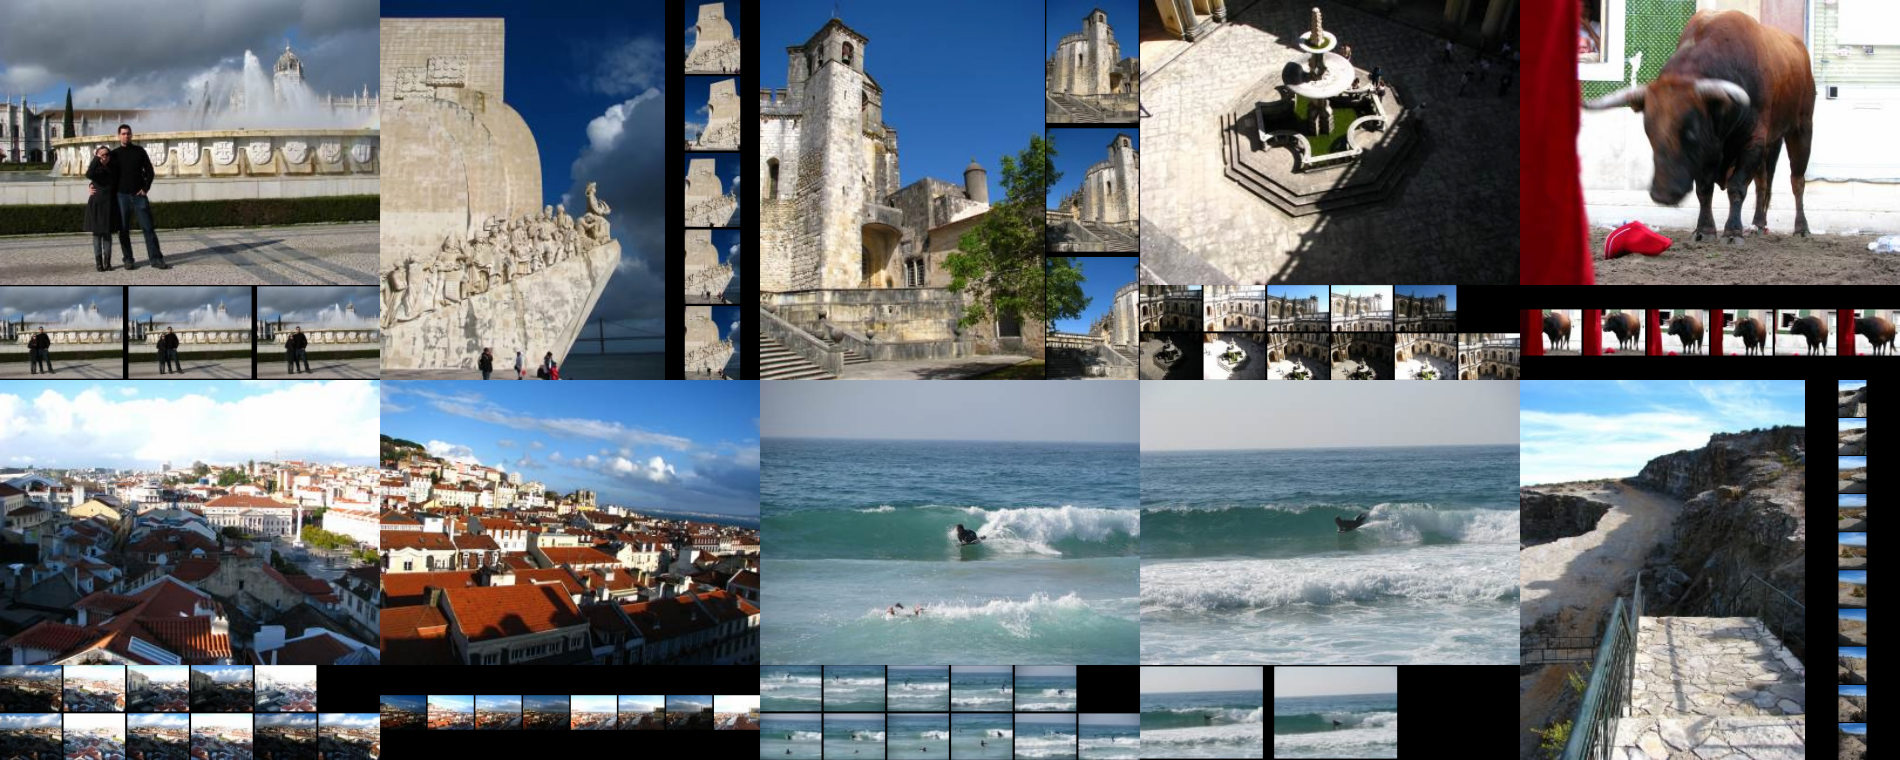
\includegraphics[width=\linewidth]{Figures/stacks-motives.png}
	\caption{Selected examples of photo stacking as presented by Eagle Eye.}
	\label{fig:stacks1}
\end{figure}

\begin{figure}[htbp]
	\centering
		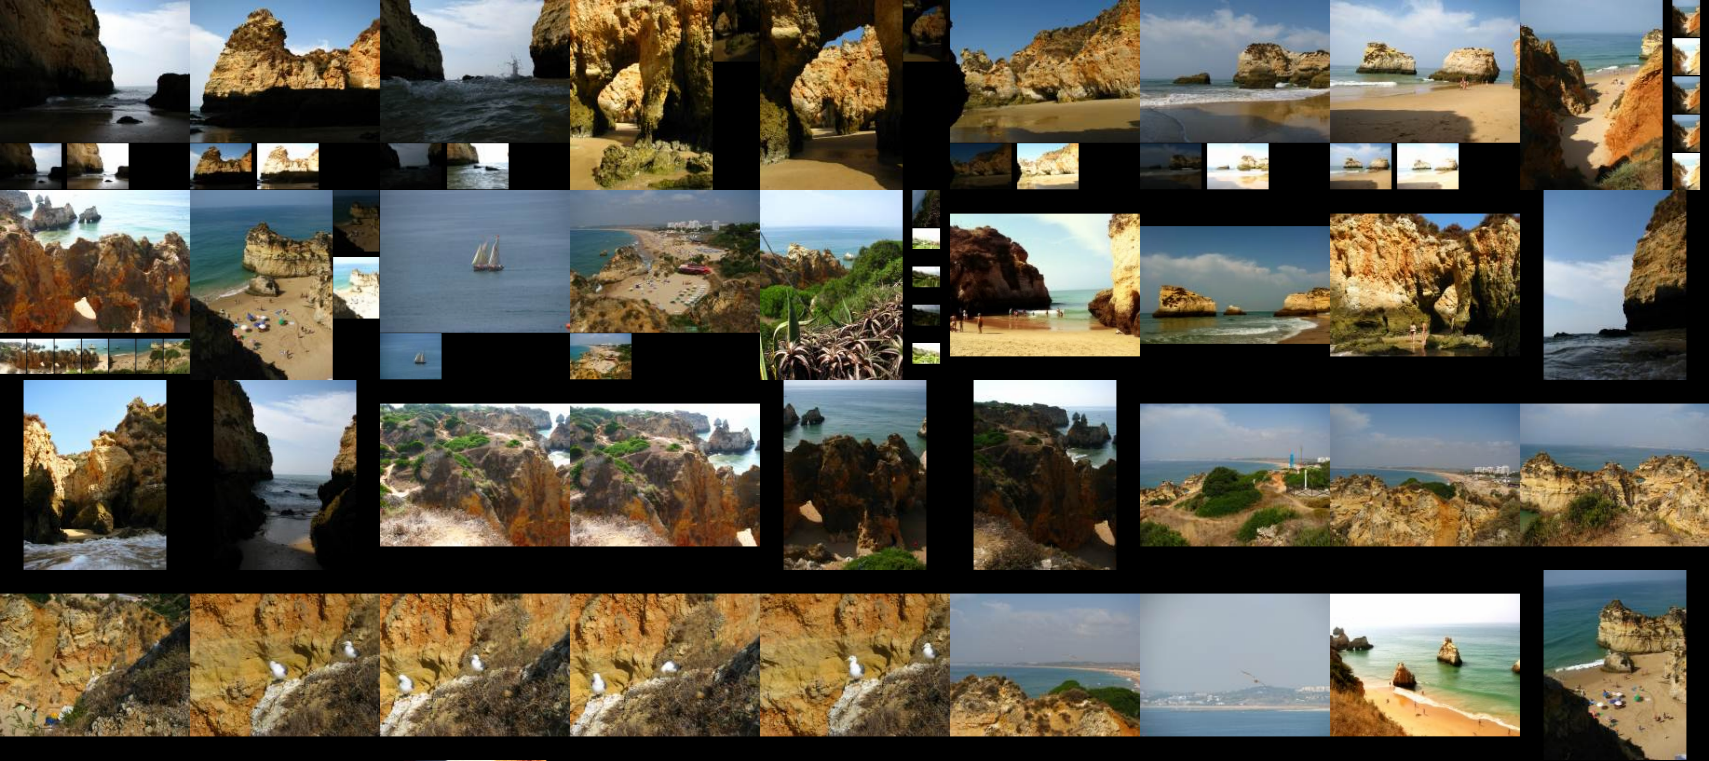
\includegraphics[width=\linewidth]{Figures/stacks-mix.png}
	\caption{Example of a trip where \ac{HDR} and Panorama techniques where applied for some photos. Other shots were repeated, some quickly and others not so much.}
	\label{fig:stacks2}
\end{figure}

Figure \ref{fig:stacks1} is a selection of success cases for this feature. It reduced a set of 80 images to just 10. It's possible to see cases where multiple pictures were taken in sequence and cases where the aim was to make a panorama. Portrait and landscape images are both equally well handled. The main image has the same size as it would be without the grouping, but is aligned to the top left corner, maximizing the free space to the left or to the bottom of the grid. This space is then filled with the other images which are adjusted in ways that can maximize their size.

Figure \ref{fig:stacks2} is a real example of a trip to the beach, where some photos were taken normally, some were taken using the \ac{HDR} or the Panorama techniques and some others where taken as a quick sequence. All this sets of photos are correctly grouped together. This figure contains a total of 71 photos, taking the space of only 36.  On the bottom left of the figure, can be see two sets of sequential photos of the same scenes that were not stacked together due to the longer period of time between their captures. To correctly group this photos in an automatic way, their visual similarity must be determined to avoid grouping unrelated photos. This is one of the features already referred on the Solution Requirements chapter (\ref{reqs:features}). 


